\documentclass[border=10pt]{standalone}
\usepackage{tikz}
\usepackage{amsmath}
\usetikzlibrary{positioning, arrows.meta}

\definecolor{vcolor}{HTML}{2E86AB}
\definecolor{mcolor}{HTML}{E8871E}
\definecolor{ccolor}{HTML}{7FB069}

\begin{document}
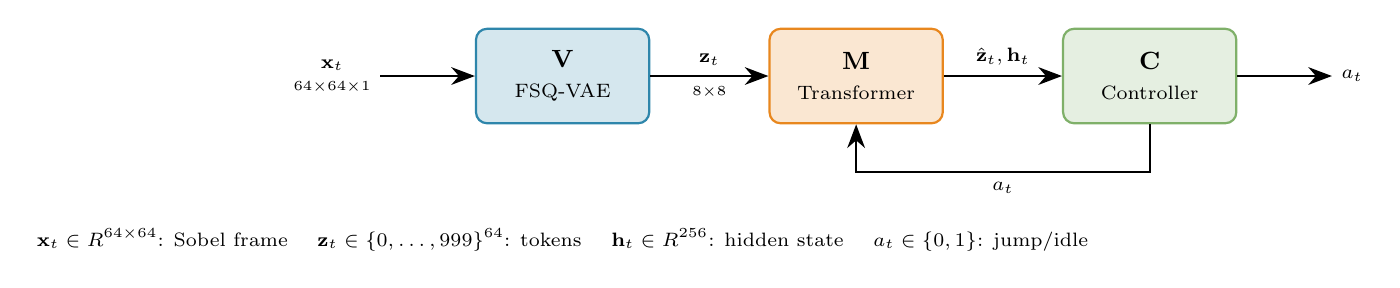
\begin{tikzpicture}[
  block/.style={rectangle, draw, rounded corners, minimum height=1.2cm, minimum width=2.2cm, align=center, font=\small, line width=0.8pt},
  arr/.style={-{Stealth[length=3mm]}, thick},
  lbl/.style={font=\scriptsize, align=center},
]
  \node[block, fill=vcolor!20, draw=vcolor] (V) {\textbf{V}\\\scriptsize FSQ-VAE};
  \node[block, fill=mcolor!20, draw=mcolor, right=1.5cm of V] (M) {\textbf{M}\\\scriptsize Transformer};
  \node[block, fill=ccolor!20, draw=ccolor, right=1.5cm of M] (C) {\textbf{C}\\\scriptsize Controller};

  \node[left=1.2cm of V, lbl] (input) {$\mathbf{x}_t$\\{\tiny 64$\times$64$\times$1}};
  \node[right=1.2cm of C, lbl] (output) {$a_t$};

  \draw[arr] (input) -- (V);
  \draw[arr] (V) -- node[above, lbl] {$\mathbf{z}_t$} node[below, lbl] {\tiny 8$\times$8} (M);
  \draw[arr] (M) -- node[above, lbl] {$\hat{\mathbf{z}}_t, \mathbf{h}_t$} (C);
  \draw[arr] (C) -- (output);

  \draw[arr] (C.south) -- ++(0,-0.6) -| node[below, lbl, pos=0.25] {$a_t$} (M.south);

  \node[below=1.2cm of V, lbl] (legend) {%
    $\mathbf{x}_t \in \mathbb{R}^{64 \times 64}$: Sobel frame \quad
    $\mathbf{z}_t \in \{0,\ldots,999\}^{64}$: tokens \quad
    $\mathbf{h}_t \in \mathbb{R}^{256}$: hidden state \quad
    $a_t \in \{0, 1\}$: jump/idle%
  };
\end{tikzpicture}
\end{document}
